\documentclass[../main.tex]{subfiles} % required, if the Chapter be a seperate doc

\begin{document}

\chapter{Messprotokolle}\label{ch:messprotokolle}

Diese Messerte wurden am \DTMdisplaydate{2025}{3}{18}{-1} in der Physiklektion durchgeführt

\section{Material}\label{sec:material}

Das ist die Liste von dem Material, welches wir für das Experiment benutzt haben

\begin{itemize}
    \item Stativ
    \item Feder 1
    \item Feder 2
    \item Konstruktionslineal
    \item Newton Messgerät (Max. 1N)
    \item Newton Messgerät (Max. 6N)
    \item 10x 10g Gewichte
    \item 2x 50g Gewichte
    \item ??? (Namen finden)
\end{itemize}
\noindent
Wir haben auch unsere Handys für documentation benutzt

\begin{figure}[ht]
    \centering
    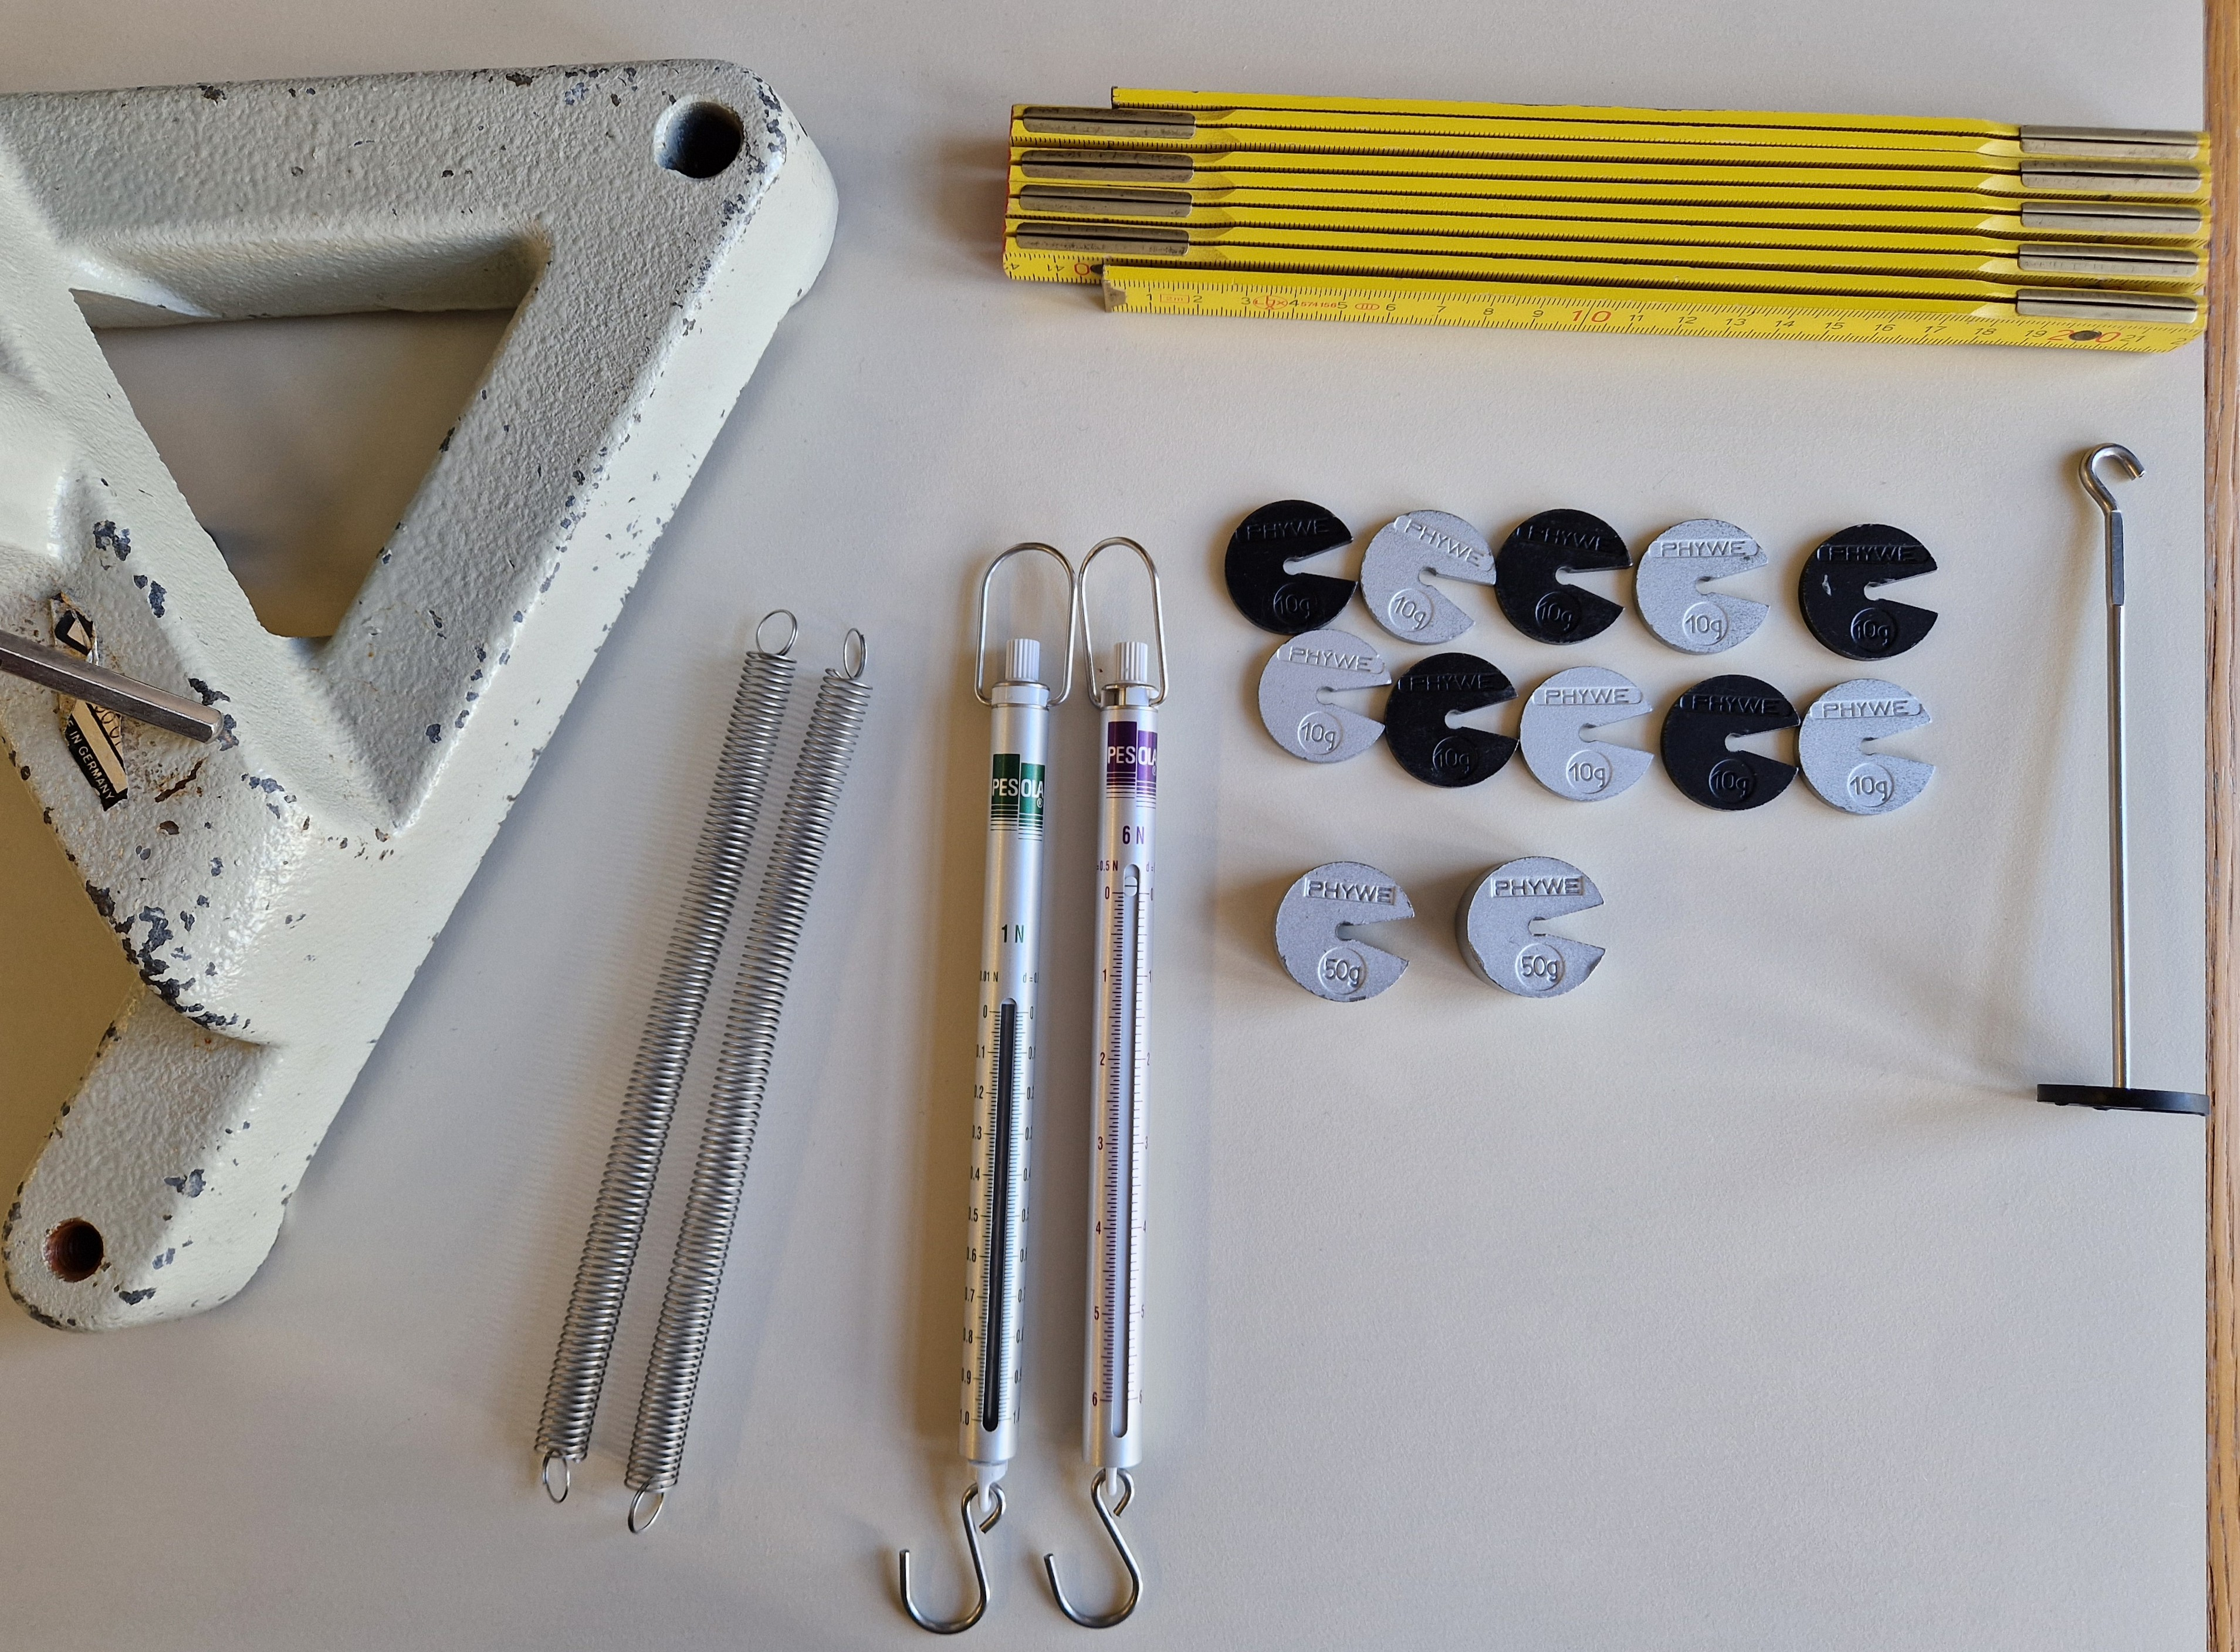
\includegraphics[width=0.7\textwidth]{Material}
    \caption{Eine Bildreferenz für das benutzte Material von dem Experiment der Datenmessung. Siehe \ref{sec:material}}
    \label{fig:material}
\end{figure}

\section{Feder 1}\label{sec:feder-1}

\begin{center}
    \begin{tabular}{ |l|l|l|l|l| } \hline\rowcolor{Gray!50}
        Index & Gewicht [g] & Mess. 1 [cm] & Mess. 2 [cm] & Mess. 3 [cm] \\\toprule\hline
        0     & 0.00        & 74.30        & 74.30        & 74.30        \\\hline
        1     & 0.01        & 73.40        & 73.50        & 73.40        \\\hline
        2     & 0.02        & 72.60        & 72.70        & 72.60        \\\hline
        3     & 0.03        & 71.80        & 71.80        & 71.80        \\\hline
        4     & 0.04        & 71.00        & 71.00        & 71.10        \\\hline
        5     & 0.05        & 70.20        & 70.10        & 70.20        \\\hline
        6     & 0.10        & 66.10        & 66.10        & 66.20        \\\hline
        7     & 0.15        & 62.00        & 62.00        & 62.10        \\\hline
        8     & 0.20        & 58.10        & 58.00        & 58.05        \\\hline
    \end{tabular}
\end{center}

\section{Feder 2}\label{sec:feder-2}

\begin{center}
    \begin{tabular}{ |l|l|l|l|l| } \hline\rowcolor{Gray!50}
        Index & Gewicht [g] & Mess. 1 [cm] & Mess. 2 [cm] & Mess. 3 [cm] \\\toprule\hline
        0     & 0.00        & 74.10        & 74.15        & 74.10        \\\hline
        1     & 0.01        & 73.30        & 73.30        & 73.30        \\\hline
        2     & 0.02        & 72.50        & 72.50        & 72.60        \\\hline
        3     & 0.03        & 71.70        & 71.70        & 71.75        \\\hline
        4     & 0.04        & 70.90        & 70.95        & 70.90        \\\hline
        5     & 0.05        & 70.10        & 70.10        & 70.10        \\\hline
        6     & 0.10        & 66.00        & 66.00        & 66.00        \\\hline
        7     & 0.15        & 62.00        & 62.00        & 61.90        \\\hline
        8     & 0.20        & 57.90        & 58.00        & 57.80        \\\hline
    \end{tabular}
\end{center}

\section{Seriell}\label{sec:seriell}

\begin{center}
    \begin{tabular}{ |l|l|l|l|l| } \hline\rowcolor{Gray!50}
        Index & Gewicht [g] & Mess. 1 [cm] & Mess. 2 [cm] & Mess. 3 [cm] \\\toprule\hline
        0     & 0.00        & 54.60        & 54.60        & 54.70        \\\hline
        1     & 0.01        & 53.00        & 53.00        & 53.00        \\\hline
        2     & 0.02        & 51.35        & 51.40        & 51.40        \\\hline
        3     & 0.03        & 49.80        & 49.80        & 49.90        \\\hline
        4     & 0.04        & 48.10        & 48.10        & 48.05        \\\hline
        5     & 0.05        & 46.40        & 46.50        & 46.40        \\\hline
        6     & 0.10        & 38.20        & 38.30        & 38.20        \\\hline
        7     & 0.15        & 30.10        & 30.20        & 30.25        \\\hline
        8     & 0.20        & 22.10        & 22.20        & 22.00        \\\hline
    \end{tabular}
\end{center}

\section{Parallel}\label{sec:parallel}

\begin{center}
    \begin{tabular}{ |l|l|l|l|l| } \hline\rowcolor{Gray!50}
        Index & Gewicht [g] & Mess. 1 [cm] & Mess. 2 [cm] & Mess. 3 [cm] \\\toprule\hline
        0     & 0.00        & 73.80        & 73.90        & 73.80        \\\hline
        1     & 0.01        & 73.60        & 73.50        & 73.40        \\\hline
        2     & 0.02        & 73.00        & 73.10        & 73.00        \\\hline
        3     & 0.03        & 72.50        & 72.60        & 72.50        \\\hline
        4     & 0.04        & 72.10        & 72.20        & 72.10        \\\hline
        5     & 0.05        & 71.70        & 71.90        & 71.70        \\\hline
        6     & 0.10        & 69.70        & 69.80        & 69.70        \\\hline
        7     & 0.15        & 67.70        & 67.90        & 67.70        \\\hline
        8     & 0.20        & 65.70        & 65.90        & 65.80        \\\hline
    \end{tabular}
\end{center}

\end{document}